\subsection{Optimum Nozzle Expansion}
Quasi 1-D Theory: The quasi 1-D theory is used for verification purposes, which assumes that all the variables are only a function of x, the below equation can be derived from invoking mass conservation and isentropic conditions\\
\begin{center}
    $(\frac{A}{A^*}) = \frac{1}{M^2}[1+\frac{\gamma-1}{2}M^2]^{\frac{\gamma+1}{\gamma-1}}$
\end{center}
\begin{figure}[H]
    \centering
    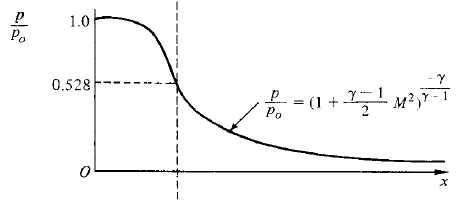
\includegraphics[width=0.5\textwidth]{text/Nozzles_Optimum.PNG}
    \caption[Variation of Pressure ratio a long center-line]{Pressure ratio vs. Center-line (Source [1])}
    \label{fig:Variation of Pressure ratio a long center-line}
\end{figure}

\begin{table}[ht]
    \centering
    \begin{tabular}{|c|c|}
    \hline
    T_{o}  &  3600 \\
    \hline
    P_{o} & 7 Mpa\\
    \hline
    P$_{e}$/P$_{th}$ & 0.0473  \\
    \hline
    A$_e$/A$_{th}$ & 3\\
    \hline
    M_{th} & 1 \\
    \hline
    M_{e} & 2.63741\\
    \hline
    P$_{e}$ & 331090.842 \\
    \hline
    T$_{e}$ & 1505.525 \\
    \hline
    \end{tabular}
    \caption{Parameters}
    \label{tab:my_label}
\end{table}

\begin{figure}[H]
    \centering
    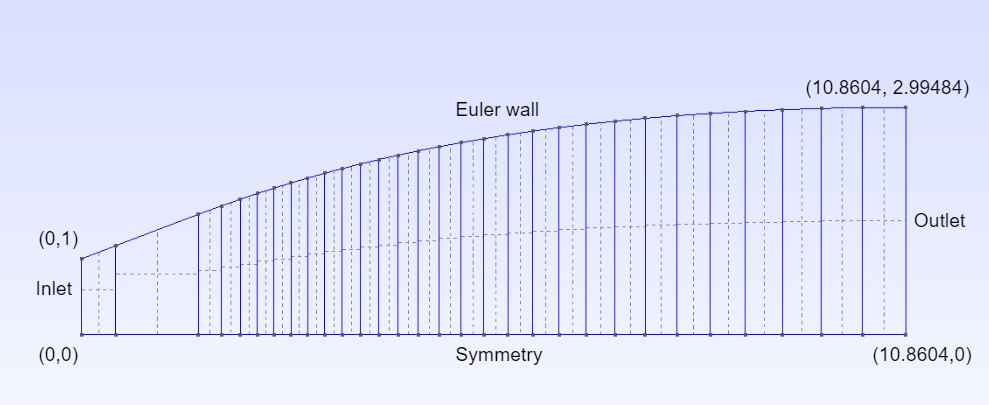
\includegraphics[width=0.75\textwidth]{text/Nozzle_Geometry.PNG}\\
    \caption[Geometry]{Geometry}
    \label{fig:Geometry}
\end{figure}
\begin{figure}[H]
    \centering
    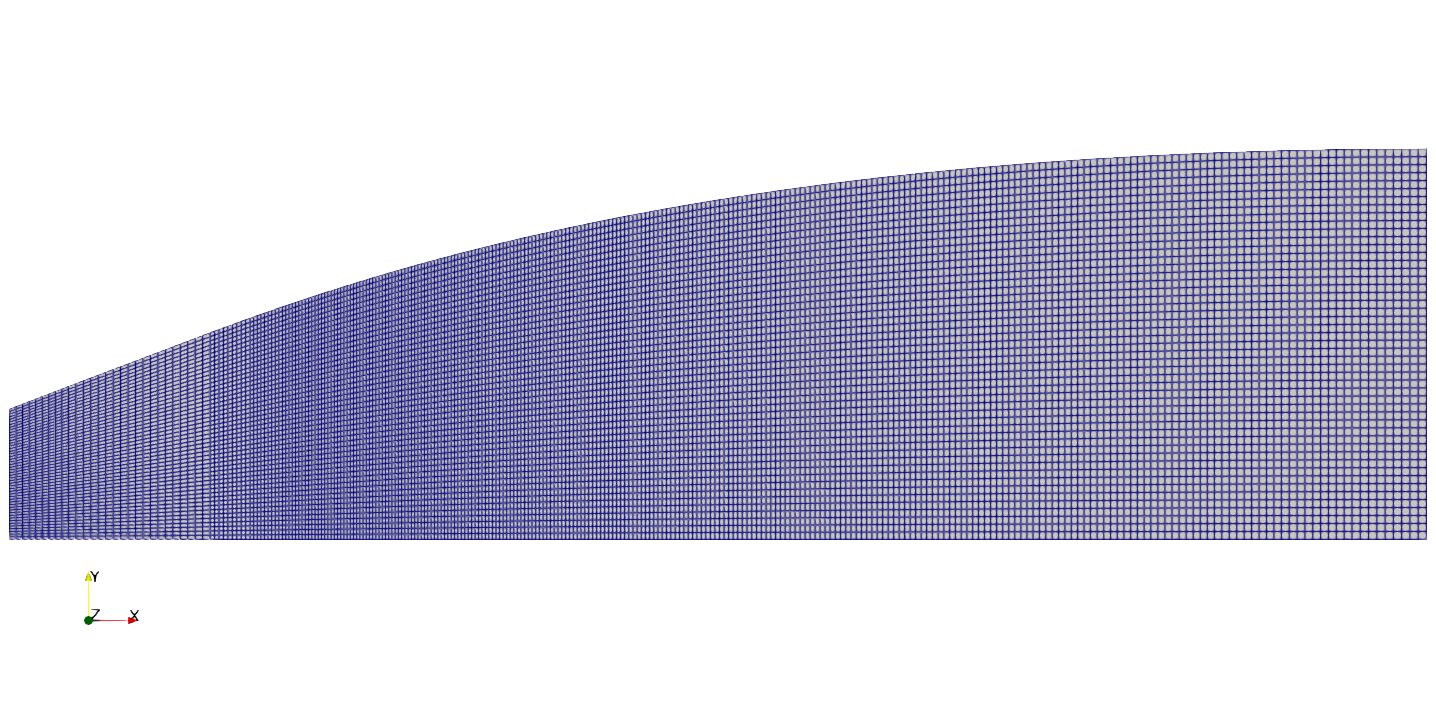
\includegraphics[width=0.8\textwidth]{text/Nozzle_mesh_pic.png}
    \caption[Mesh]{Mesh}
    \label{fig:Mesh}
\end{figure}

\begin{flushleft}
\textbf{Set-Up}\\
\end{flushleft}
\begin{center}
\begin{tabular}{|l|l|}
     \hline
     Solver & Euler  \\
     \hline
     Num\_Method\_Grad & Weighted\_Least\_Squares  \\
     \hline
    Conv\_Num\_Method\_Flow & \textbf{JST}  \\
     \hline
    CFL & 5\\
     \hline
     Time\_Diecre\_Flow & Euler\_Implicit\\
     \hline
    Conv\_Field & RMS\_Density\\
     \hline 
    Conv\_Residual\_Minval & -12 (log_1_0)\\
     \hline 
    Conv\_Cauchy\_Eps & 1E-10 (last 100 elements)\\
     \hline
\end{tabular}\\
\end{center}
\\
\\
\textbf{Initial Condition}\\
Mach$_{free-stream}$ = 1 also serves as the initial condition. In this case, this is valid as the mach number inside the nozzle is always greater than 1.\\
\\
\textbf{Solver \& Convective Numerical Scheme}\\
Euler solver is used with JST convective numerical scheme. Other than JST and Lax-Friedrich scheme only ROE scheme showed convergence with high multigrid option. Other schemes either diverged or didn't converge. The cauchy convergence criteria is used, the average of the last 100 log$_1_0$(density residual) is set less than -12 for convergence. \\
%\end{flushleft}
%The chamber temperature and pressure is 3600 k and 7 MPa. The ratio of A$_e$/A$_t$ is 3:1. The inlet is the throat with speed of flow as M = 1. The outlet pressure is 331090.842 Pa, temperature is 1505.525 and mach number is 2.63741 as calculated using the quasi 1-D theory. Air is chosen and the gas is assumed to be ideal, hence, specific heat ratio is 1.4 and gaseous constant is 287.
\\
\textbf{Grid Independent Test}\\
\begin{table}[ht]
    \centering
    \begin{tabular}{|c|c|c|c|c|c|c|c|}
    \hline
    No of Elements & M$_e$ & P$_e$ & T$_e$ & M$_{error}$ & P$_{error}$ & T$_{error}$ & Time\\
    \hline
       73755(S)  & 2.63818 & 330742 & 1505.02 & 0.045 & 0.106 & 0.034 & 580s\\
       \hline
       13720(S)  & 2.63973 & 330060 & 1504.03 & 0.104 & 0.311 & 0.100 & 53s\\
       \hline
       7630(S)   & 2.64024 & 329909 & 1503.73 & 0.123 & 0.357 & 0.120 & 25s\\
       \hline
       26324(US)   & 2.63607 & 331749 & 1506.42 &  0.051 & 0.2 & 0.120 & 75s\\
       \hline
       7053(US)   & 2.63435 & 332671 & 1507.56 & 0.116 & 0.478 & 0.135 & 10s\\
       \hline
    \end{tabular}
    \caption{S is Structured and US is Unstructured Grid}
    \label{tab:Grid Independent Test}
\end{table}
\begin{figure}[H]
    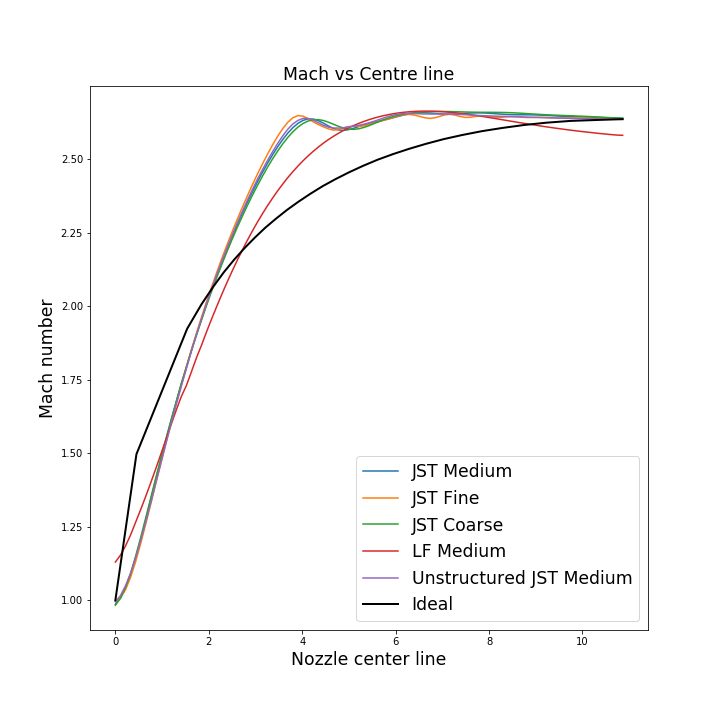
\includegraphics[width=0.5\textwidth]{text/Mach_vs_X.png}
    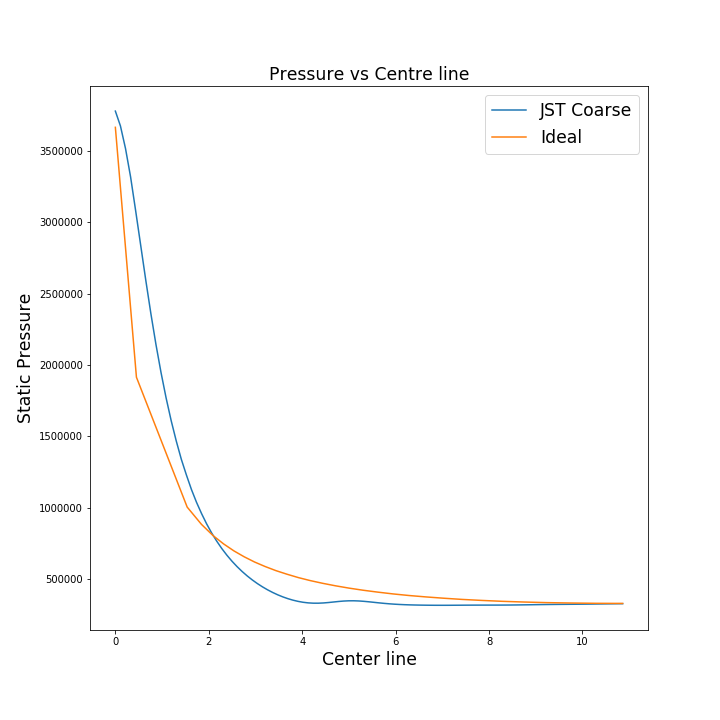
\includegraphics[width=0.5\textwidth]{text/Pressure_vs_X.png}
    \caption[Error along Center line]{Error along Center line}
    \label{fig:Error along Center line}
\end{figure}
\begin{flushleft}
\textbf{Conclusion}
\end{flushleft}
\vspace{-5}
Even though the exit parameters from the simulation are close enough to the values calculated from the quasi 1-D theory, the values in between the inlet and outlet show considerable deviation. \\
\begin{figure}[H]
    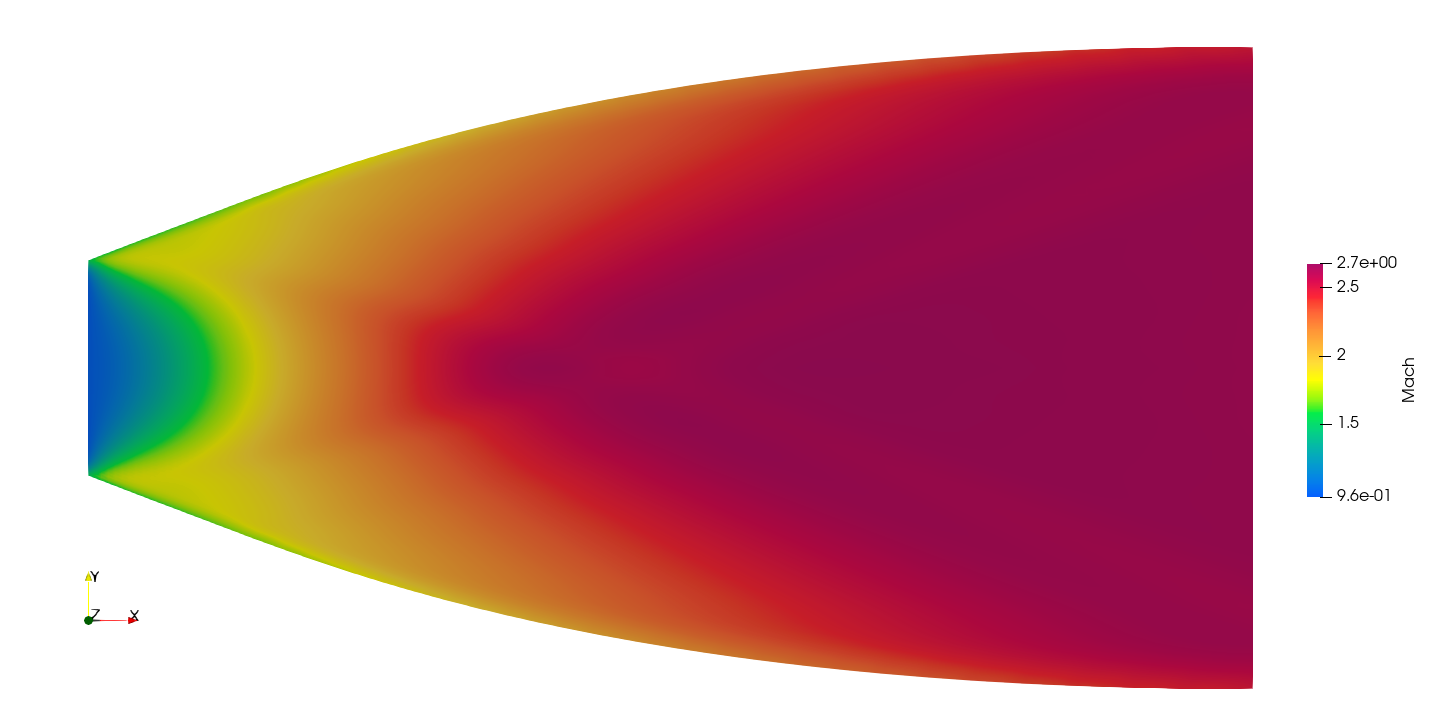
\includegraphics[width=0.5\textwidth]{text/Coarse_JST_Mach.png}
    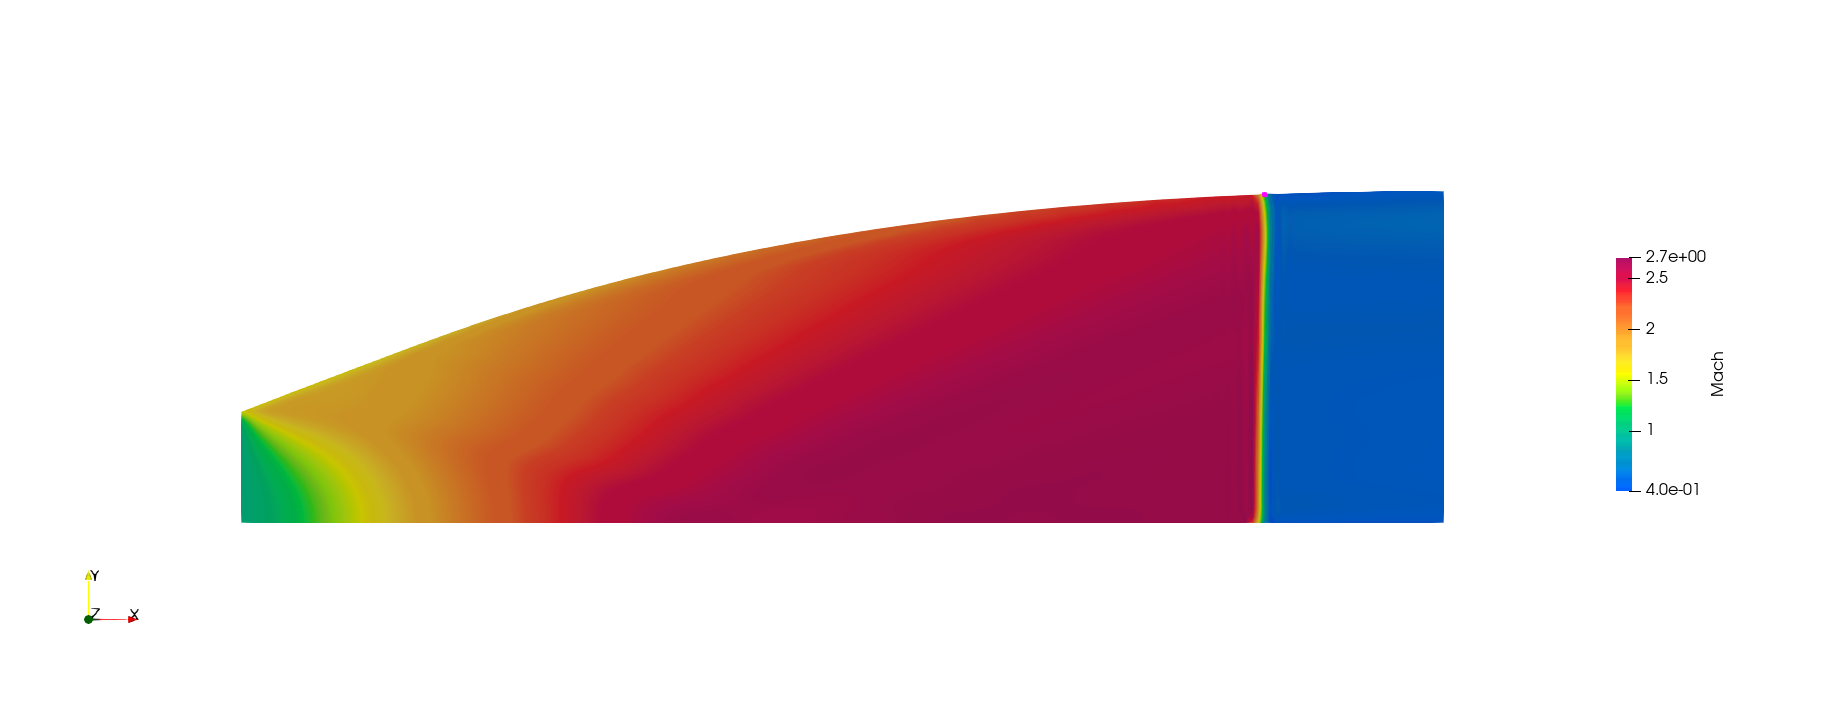
\includegraphics[width=0.5\textwidth]{text/NS_Loc.png}
    \caption[Mach Contour of flow through nozzle]{Mach Contour using JST Scheme}
    \label{fig:Mach Contour using JST Scheme}
\end{figure}

\newpage
\subsection{Extended Nozzle Simulations}
\textbf{Theory}\\
\begin{figure}[H]
    \centering
    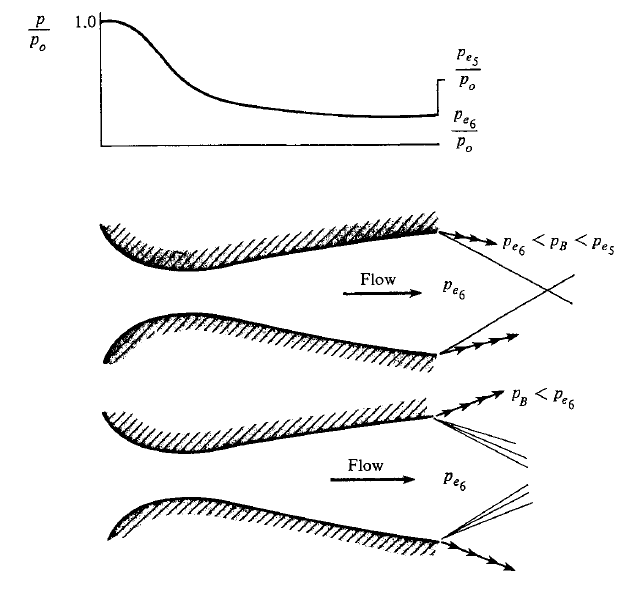
\includegraphics[width=0.6\textwidth]{text/Nozzles_Expansions.PNG}
    \caption[Over-expanded and Under-expanded Nozzle]{Over-expanded and Under-expanded Nozzle (Source [1])}
    \label{fig:Over-expanded and Under-expanded Nozzle}
\end{figure}
\textbf{Geometry}\\
\begin{figure}[H]
    \centering
    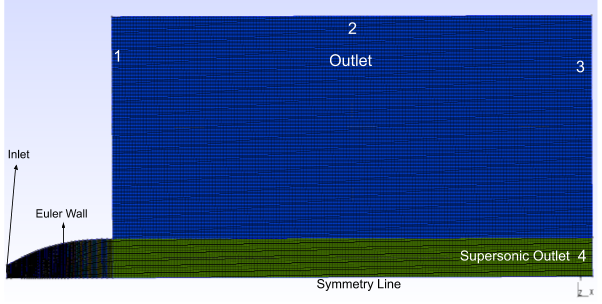
\includegraphics[width=0.75\textwidth]{text/Failed_BC.png}
    \caption[Extended Mesh of Nozzle Simulation]{Mesh}
    \label{fig:Mesh}
\end{figure}
\begin{flushleft}
\textbf{Impact of Boundary Conditions \& Initial Conditions on the Result}
\end{flushleft}
For an optimum expanded nozzle the \textbf{Outlet} is assigned a back-pressure that equals P$_{e6}$. The is a \textbf{pressure outlet} boundary condition. Since there is no velocity inlet option for compressible flows, P$_0$ and T$_0$ are assigned at the inlet. For a rocket engine that is just about to start the natural initial condition is that the speed is zero everywhere and the pressure is P$_{e6}$ and temperature is same as the atmospheric temperature. There is \textbf{NO OPTION} in SU2 to simultaneously assign Mach 1 at the inlet and Mach 0 to the rest of the domain as the initial conditions. This simulation always resulted in divergent issues or the residual oscillates continuously without a proper velocity field. To solve this issue several approaches were tried out.\\
\\
(A) Supersonic Outlet:The outlet which would have supersonic flow is given outlet supersonic. Other outlets have atmospheric pressure as the BC. The atmospheric pressure is same as the nozzle outlet pressure for optimum expansion of the nozzle. \\
\begin{figure}[H]
    \centering
    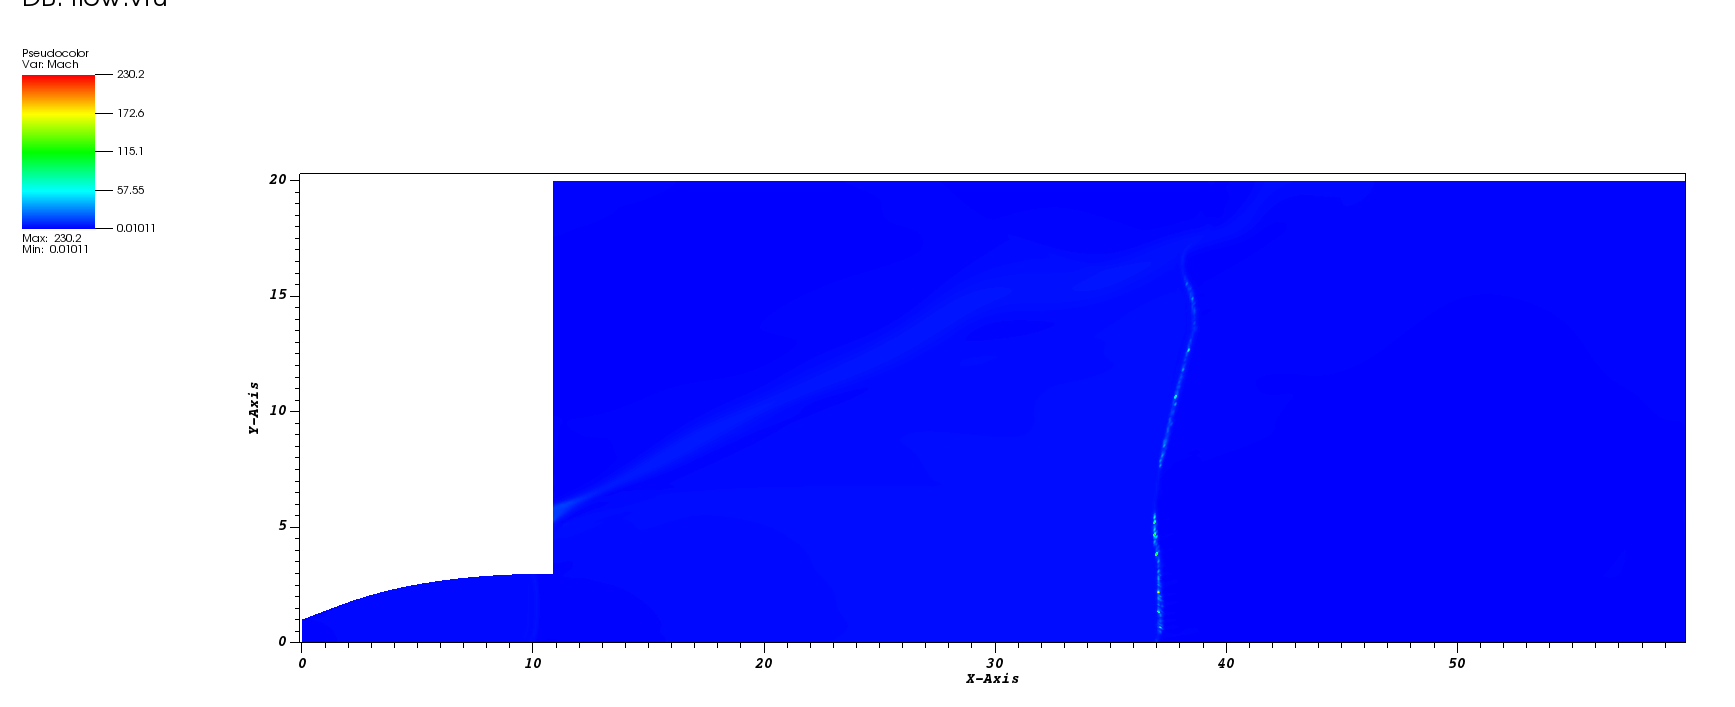
\includegraphics[width=0.55\textwidth]{text/F1.png}
    \caption[Mach Contour of Extended Mesh I]{Mach Contour}
    \label{fig:Mach Contour}
\end{figure}
The simulation resulted in residuals that oscillated continuously. diverged residuals. Different CFL values were used in the simulation, but none yielded the desired results.\\
\\
(B) Free-stream Conditions: The initial condition throughout the domain is assigned the free-stream values as shown\\
FREESTREAM\_PRESSURE = 3697972.51402 Pa\\
FREESTREAM\_TEMPERATURE = \textcolor{red}{3000 K} \\
\begin{figure}[H] 
    \centering
    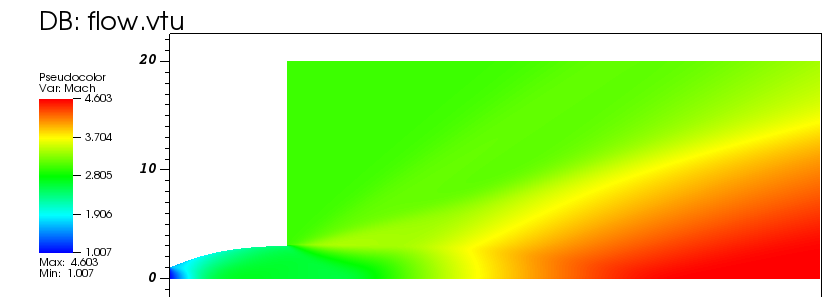
\includegraphics[width=0.75\textwidth]{text/Mach contour 1.png}
    \caption[Mach Contour of Extended Mesh II]{Mach Contour}
    \label{fig:Mach Contour}
\end{figure}
Though the exit parameters match the required optimum conditions, due to the incorrect initial conditions at the domain outside the nozzle the flow develops expansion fans.\\
\\
\\
(C) Optimum Expanded Nozzle: The \textbf{pressure outlet} boundary condition is replaced as \textbf{farfield}. The freestream values are P$_{e6}$ and atmospheric temperature \textcolor{red}{3000 K}\\
\begin{figure}[H]
    \centering
    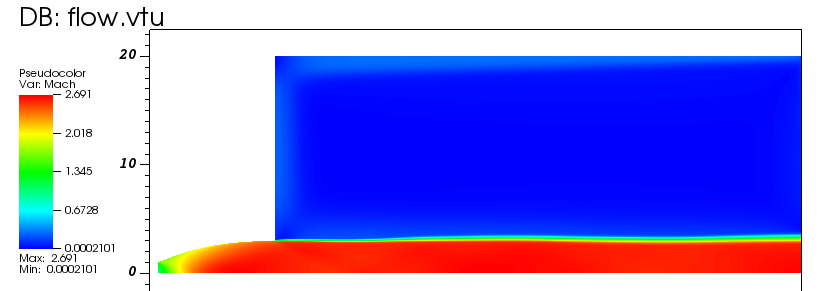
\includegraphics[width=0.75\textwidth]{text/Mach_ROE_Success.png}
    \caption[Mach Contour of Extended Mesh III]{Mach Contour}
    \label{fig:Mach Contour}
\end{figure}
\begin{table}[ht]
    \centering
    \begin{tabular}{|c|c|}
    \hline
    T_{o}  &  3600 \\
    \hline
    P_{o} & 7 Mpa\\
    \hline
    P$_{e}$/P$_{th}$ & 0.0473  \\
    \hline
    \end{tabular}
    \caption{Parameters}
    \label{tab:my_label}
\end{table}
\\
(D) Under-Expanded Nozzle: he \textbf{pressure outlet} boundary condition is \textbf{farfield}. The freestream values are P$_{exit}$ = 1 atm and atmospheric temperature \textcolor{red}{3000 K}
\begin{figure}[H]
    \centering
    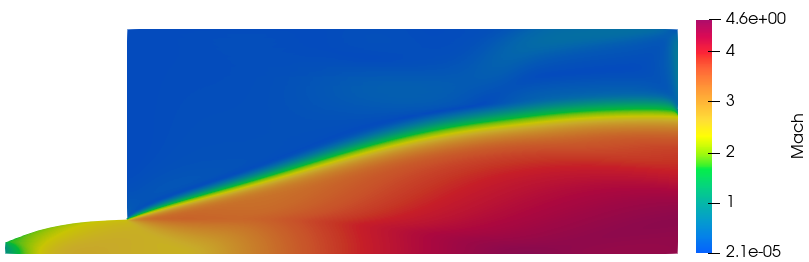
\includegraphics[width=0.75\textwidth]{text/Mach_Underexpanded Nozzle.png}
    \caption{Mach Contour Under-Expanded Nozzle}
    \label{Mach Contour Under-Expanded Nozzle}
\end{figure}
The initial condition on temperature seems to be the crucial parameter as it produces converging residuals. Altering this value to any other value either gives unsteadiness in the flow or produces viscous like effect. \\

(E) Under-Expanded Nozzle: he \textbf{pressure outlet} boundary condition is \textbf{farfield}. The freestream values are P$_{exit}$ = 500000 Pa and atmospheric temperature \textcolor{red}{3000 K}
\begin{figure}[H]
    \centering
    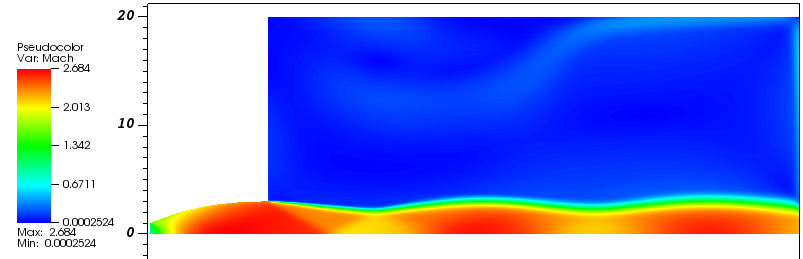
\includegraphics[width=0.75\textwidth]{text/Mach_Overexpanded Nozzle.png}
    \caption{Mach Contour Over-Expanded Nozzle}
    \label{Mach Contour Over-Expanded Nozzle}
\end{figure}

\newpage
\begin{flushleft}
\textbf{Results and Analysis}\\
\end{flushleft}
The initial condition for temperature is strictly incorrect for the entire domain that is present outside the nozzle as the temperature outside the nozzle is just 288 kelvin and pressure is P$_{e6}$. But the prime reason to take this approach is to ensure that the inlet initial condition meets the required mach number, i.e., 1. There is no clear picture to understand how SU2 calculates the inlet mach number with the given boundary conditions and initial condition. One hypothesis is that with the given total conditions SU2 might assume isentropic flow and it evaluates the mach number as 2.64 at the outlet. This value may be used to back calculate the mach number at the inlet. But when the free-stream temperature is assigned 288 K, the residual starts to \textbf{oscillate}. One hypothesis could be the Mach number which is calculated from P$_{e6}$ and T$_0$ must be same for physical consistency.\\
\newpage